%
\hsection{Entities and Attributes}%
\label{sec:entitisAttrsErd}%
%
The first major component to model are the datastructures to be stored inside the \db.
For this purpose, the following modeling primitives have emerged.
The most basic elements for conceptual modeling are entities, attributes, and entity types.%
%
\begin{definition}[Entity]%
\label{def:entity}%
An \emph{entity} is an object or thing with an independent existence in the world. %
It can be distinguished from all other objects.%
\end{definition}%
%
Examples of entities are maybe the student Mr.~Bibbo, the module~\citetitle{programmingWithPython}~\cite{programmingWithPython}, the professor Mrs.~Bebba~教授, room~\#36~305, or the curriculum \emph{Computer Science and Technology}.
Entities can be spotted easily in the requirement specification or when viewing the meeting or interview notes:
They correspond to \emph{proper nouns}~\cite{S2024D:CDMERDE}, i.e., nouns that actually name one specific thing and that are usually capitalized~\cite{EOWM2025MWAMTD:CAPNWTDLWOGC}.%
%
\begin{definition}[Attribute]%
An \emph{attribute} is a feature or characteristic of an entity.%
\end{definition}%
%
Entities in our model are represented by the values of their attributes.
A student could be defined by their name, ID, student~ID, mobile phone number, home address, date of birth, etc.
A module could be described by its title, syllabus, and abstract.
Additionally to such features, \emph{adjectives} in the requirements text often can be interpreted as attribute values, e.g., red, young, successful, heavy, fast.%
%
\begin{definition}[Domain]%
The \emph{domain} of an attribute is the set of possible values that it can take on.%
\end{definition}%
%
The name of a student is a text string.
The mobile phone numbers and IDs may be a text strings, too, but of a fixed length and limited to certain character ranges at certain positions.
The \pgls{dateOfBirth}, on the other hand, is a date.
The score in an exam may be an integer number between~0 and~100.%
%
\begin{definition}[Entity Type]%
\label{def:entityType}%
The set of all entities that have the same attributes is called an \emph{entity type}.%
\end{definition}%
%
So while the entity Mr.~Bebbo is a single student, the set of all possible students would form an entity type.
While the module~\citetitle{programmingWithPython}~\cite{programmingWithPython} is a single entity, the set of all possible modules would form an entity type.
Mrs.~Bebba~教授 is a single entity, but the set of all possible professors represents an entity type.
Entity types are \emph{common nouns} that stand for groups or types of things~\cite{S2024D:CDMERDE} and that are usually written with lowercase letters~\cite{EOWM2025MWAMTD:CAPNWTDLWOGC}.

Also notice the plural \emph{attributes} in \cref{def:entityType}:%
\bestPractice{entityTypesHaveMultipleAttributes}{%
Only things with multiple attributes should become entity types.%
}%
Indeed, it makes little sense, for example, to consider \emph{year} as an entity type, because it does not have multiple attributes.%
%
\begin{definition}[Entity Set]%
An \emph{entity set} is a subset of an entity type. %
It is a set of some entities of a type that exist at one point in time.%
\end{definition}%
%
For example, Mr.~Bebbo is a single student entity, the set of all possible student entities forms an entity type, but the students Mr.~Bebbo, Mr.~Bibbo, and Mr.~Bobbo together form an entity set.
The modules~\citetitle{programmingWithPython}~\cite{programmingWithPython} and \citetitle{databases}~\cite{databases} form an entity set, because they are a subset of an entity type for modules.
Notice that the mathematical notion of \emph{set} is indeed correct here:
All entities have a unique identity and, hence, can be differentiated from all possible other objects.
There are no two identical Mr.~Bibbos.
Therefore, students can be grouped in a set and entity types are sets, too.

Viewing the conceptual design of \dbs\ through this lense, we notice a few things.
First, we always model only a tiny window to the real world.
When we talk about students, modules, and curricula as entity types, this only concerns our particular application.
Of course, in our real big wide world, students exist in other universities and in other countries.
These students may have completely different attributes from ours.
They do not matter in the model of our small part of the world.

Second, if you attended or do attend a course on programming, then you will feel that this way of modeling things is a bit related to \pgls{OOP}.
Entity types could be thought of as \pythoniles{class}, entities could be their instances and attributes could be their, well, attributes.
While \db\ theorists may dislike this way of thinking, I believe that it is not wrong.
It is a viable analogy.
However, later, when we model the relationships between entities, it may no longer be helpful.

We now know that entity types with their attributes basically correspond to datastructures in programming.
They form one element of the conceptual model.
But how do we actually write them down?
How do we specify them?

For this, a graphical notation has been introduced:
\glsreset{ERD}\Pglspl{ERD} are the most commonly used tool to model the entity types and their relationships in a \db~\cite{C2002ERMHEFTALL,C1975TRMTAUVOD,C1976TERMTAUVOD,KW2012ASHOTEDAIM,WF1995DHQDM,B1990CMERMO}.
There exists a wide variety of graphical notations that can be used for \pglspl{ERD}.
The original notations by \citeauthor{B1969DSD}~\cite{B1969DSD} and \citeauthor{C1975TRMTAUVOD}~\cite{C1975TRMTAUVOD,C1976TERMTAUVOD} are still in use, the more comprehensive and standardized \pgls{IDEF1X} syntax~\cite{FIPSPUB184,ISOIECIEEE2012ITMLP2SASFII}, and the \glsreset{UML}\pgls{UML}~\cite{OMG2017OUMLOU,RMHOSMUUIIIIOPPTRS1997UNG,BRJ1999TUMLRM}.
Indeed, there are many different flavors of diagrams that can serve as \pglspl{ERD}.
\Citeauthor{S2024D:CDMERDE}~\cite{S2024D:CDMERDE}, for example, presents nine slightly different variations.
\Citeauthor{SS2005EIDDDFDB:CDDRAAML}~\cite{SS2005EIDDDFDB:CDDRAAML} has two baseline variants, including several slight variations of a \pgls{UML}-based approach~(which is not listed in~\cite{S2024D:CDMERDE}).
The notation used by \citeauthor{V1999C5DMS:CDUTERM}~\cite{V1999C5DMS:CDUTERM} is yet again slightly different.
Therefore, \pglspl{ERD} may look slightly different depending on who drew them and which tools they used.
However, understanding them is not really hard, so these differences are not that important.

\begin{figure}%
\centering%
%
\subfloat[][%
We open the \yEd\ editor and click on the \menu{Entity Relationship} tab in the \menu{Palette} view on the right-hand side.%
\label{fig:yedErdEntitiesA01scrollToErd}%
]{\tightbox{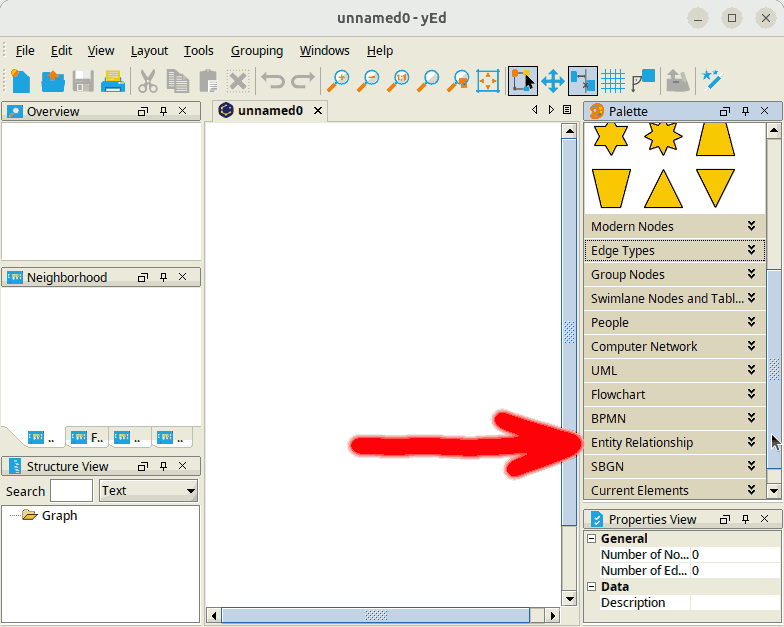
\includegraphics[width=0.48\linewidth]{\currentDir/yedErdEntitiesA01scrollToErd}}}%
%
\floatSep%
%
\subfloat[][%
We can now click on the \menu{Entity} symbol and drag it into the empty document.%
\label{fig:yedErdEntitiesA02entity}%
]{\tightbox{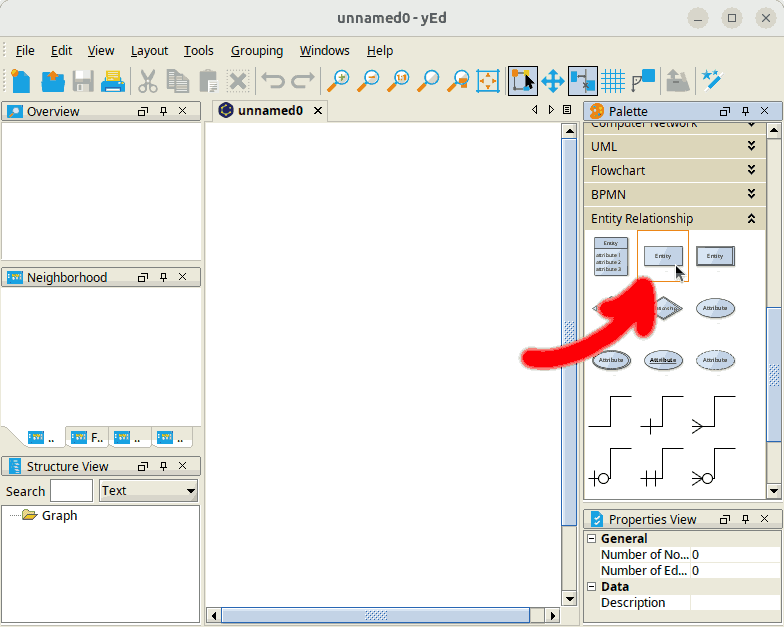
\includegraphics[width=0.48\linewidth]{\currentDir/yedErdEntitiesA02entity}}}%
%
\floatRowSep
%
\subfloat[][%
We dragged the entity symbol into the diagram document.%
\label{fig:yedErdEntitiesA03dragEntity}%
]{\tightbox{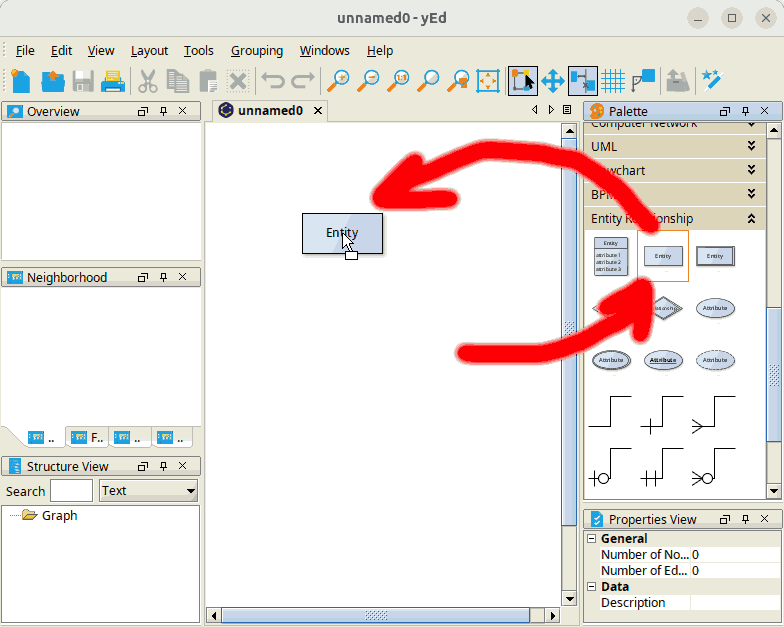
\includegraphics[width=0.48\linewidth]{\currentDir/yedErdEntitiesA03dragEntity}}}%
%
\floatSep
%
\subfloat[][%
We double-click into the new entity symbol in order to edit its name.%
\label{fig:yedErdEntitiesA04doubleClickName}%
]{\tightbox{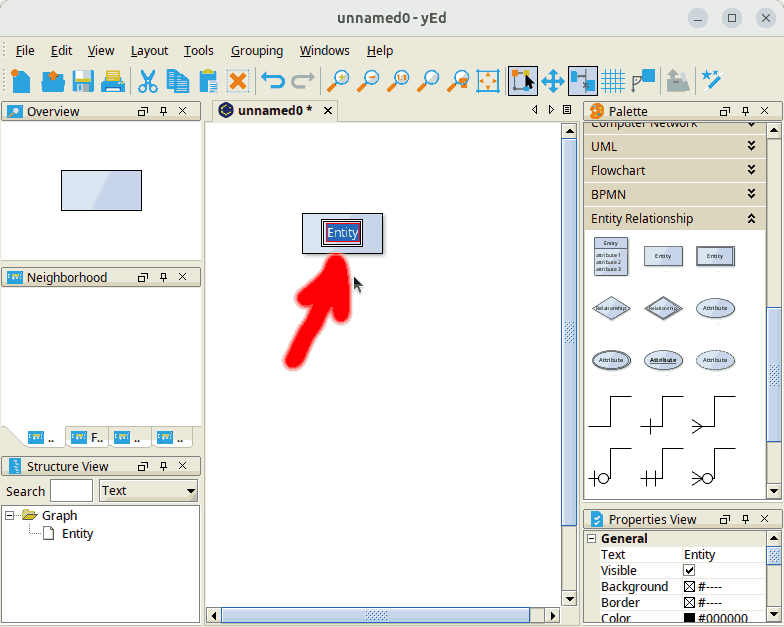
\includegraphics[width=0.48\linewidth]{\currentDir/yedErdEntitiesA04doubleClickName}}}%
%
\floatRowSep
%
\subfloat[][%
We change the entity name to \inQuotes{Student} and press \keys{\enter}.%
\label{fig:yedErdEntitiesA05changeNameToStudent}%
]{\tightbox{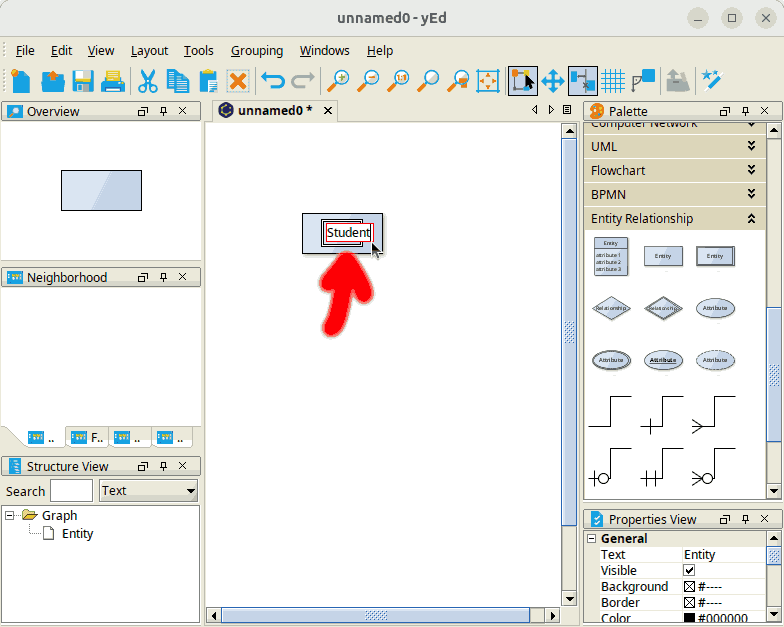
\includegraphics[width=0.48\linewidth]{\currentDir/yedErdEntitiesA05changeNameToStudent}}}%
%
\floatSep
%
\subfloat[][%
The name has changed. We now click on the \menu{Attribute} symbol in the element palette.%
\label{fig:yedErdEntitiesA06nameIsStudentSelectAttribute}%
]{\tightbox{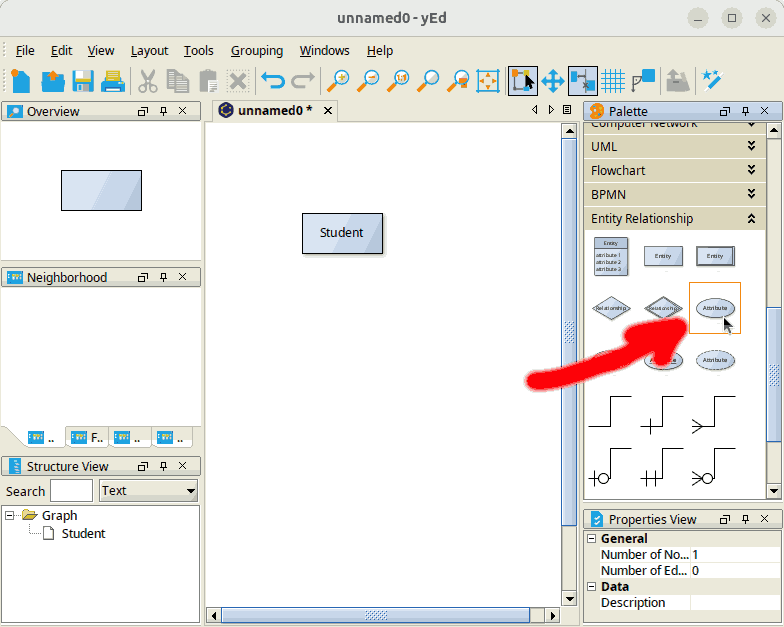
\includegraphics[width=0.48\linewidth]{\currentDir/yedErdEntitiesA06nameIsStudentSelectAttribute}}}%
%
\caption{Drawing an \pgls{ERD} for the \emph{Student} entity using \yEd.}%
\label{fig:yedErdEntitiesA:A}%
\end{figure}%
%
\begin{figure}%
\ContinuedFloat%
\centering%
%
\subfloat[][%
We drag the attribute symbol into our document.%
\label{fig:yedErdEntitiesA07dragAttribute}%
]{\tightbox{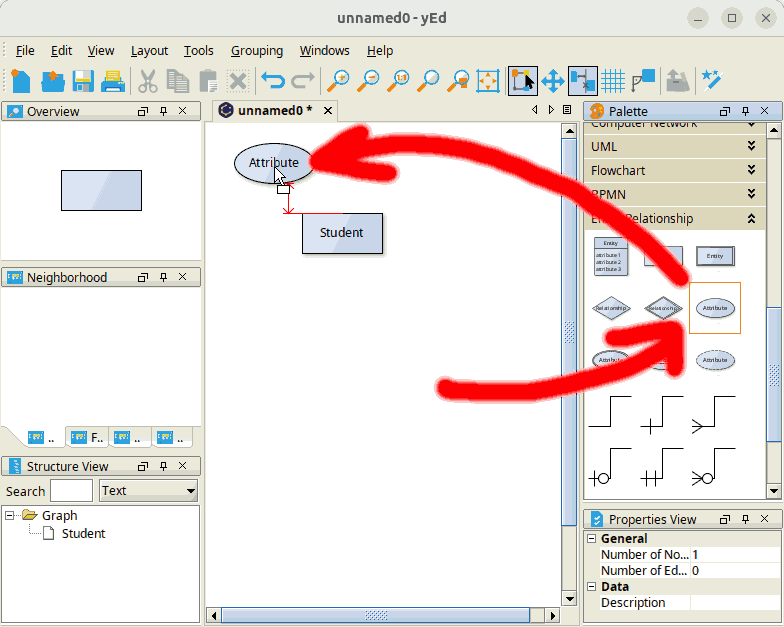
\includegraphics[width=0.48\linewidth]{\currentDir/yedErdEntitiesA07dragAttribute}}}%
%
\floatSep%
%
\subfloat[][%
We double-click into it to change its name.%
\label{fig:yedErdEntitiesA08doubleClickName}%
]{\tightbox{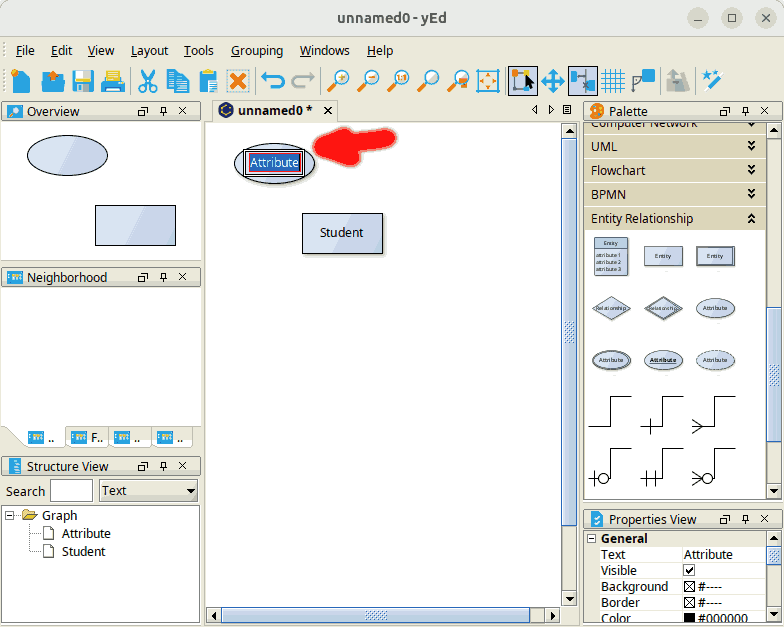
\includegraphics[width=0.48\linewidth]{\currentDir/yedErdEntitiesA08doubleClickName}}}%
%
\floatRowSep
%
\subfloat[][%
We want its name to be, well, \inQuotes{Name.}%
\label{fig:yedErdEntitiesA09changeNameToName}%
]{\tightbox{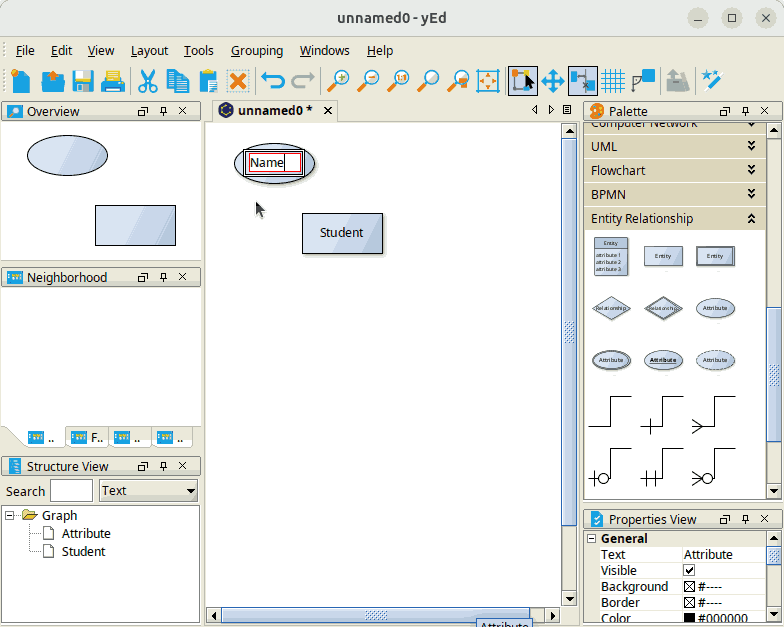
\includegraphics[width=0.48\linewidth]{\currentDir/yedErdEntitiesA09changeNameToName}}}%
%
\floatSep
%
\subfloat[][%
We changed the attribute name. %
Now we click on the connection symbol in the palette and drag it right onto the attribute.%
\label{fig:yedErdEntitiesA10changeNameChangedToNameSelectConnection}%
]{\tightbox{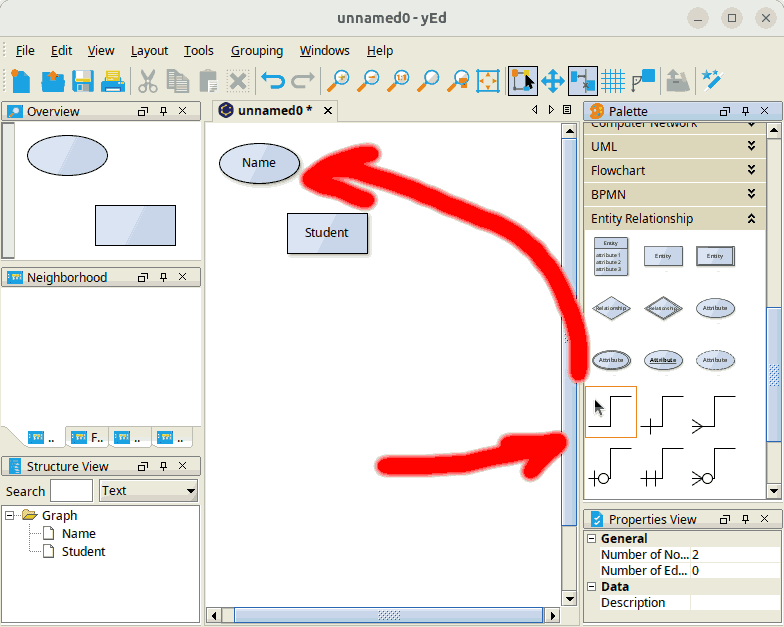
\includegraphics[width=0.48\linewidth]{\currentDir/yedErdEntitiesA10changeNameChangedToNameSelectConnection}}}%
%
\floatRowSep
%
\subfloat[][%
We drop the connection symbol onto the \emph{Name} attribute.%
\label{fig:yedErdEntitiesA11dragConnection}%
]{\tightbox{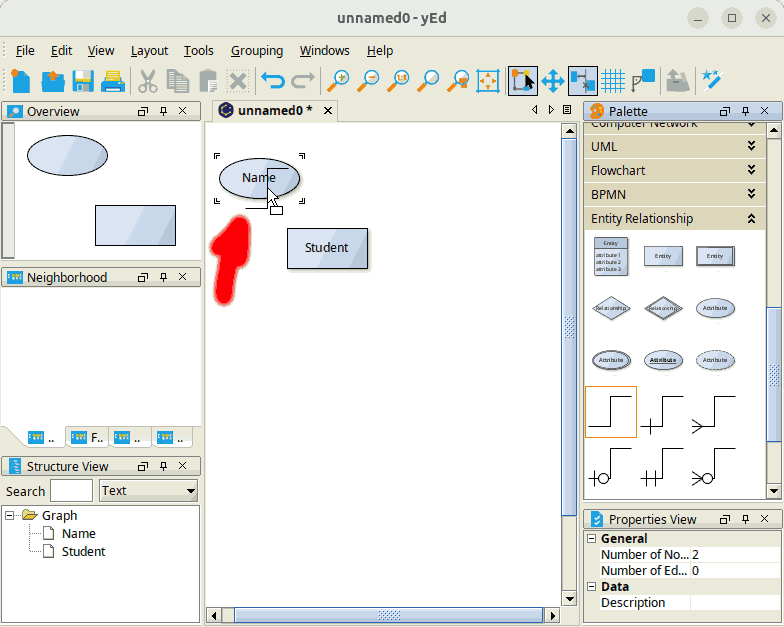
\includegraphics[width=0.48\linewidth]{\currentDir/yedErdEntitiesA11dragConnection}}}%
%
\floatSep
%
\subfloat[][%
We then click into the entity to connect the attribute \emph{Name} to the \emph{Student} entity.%
\label{fig:yedErdEntitiesA12connectToStudent}%
]{\tightbox{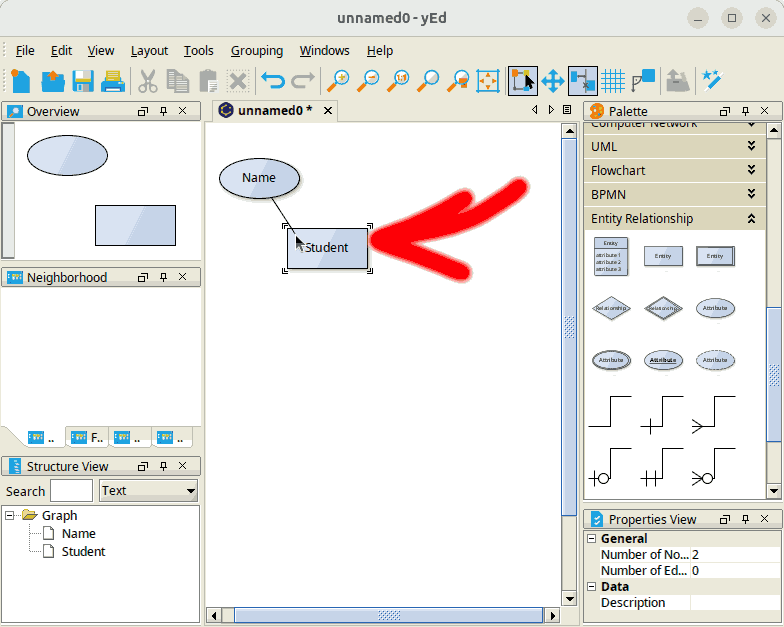
\includegraphics[width=0.48\linewidth]{\currentDir/yedErdEntitiesA12connectToStudent}}}%
%
\caption{Drawing an \pgls{ERD} for the \emph{Student} entity using \yEd~(Continued).}%
\label{fig:yedErdEntitiesA:B}%
\end{figure}%
%
\begin{figure}%
\ContinuedFloat%
\centering%
%
\subfloat[][%
The \emph{Name} attribute is now connected to the \emph{Student} entity.%
\label{fig:yedErdEntitiesA13connectedToStudent}%
]{\tightbox{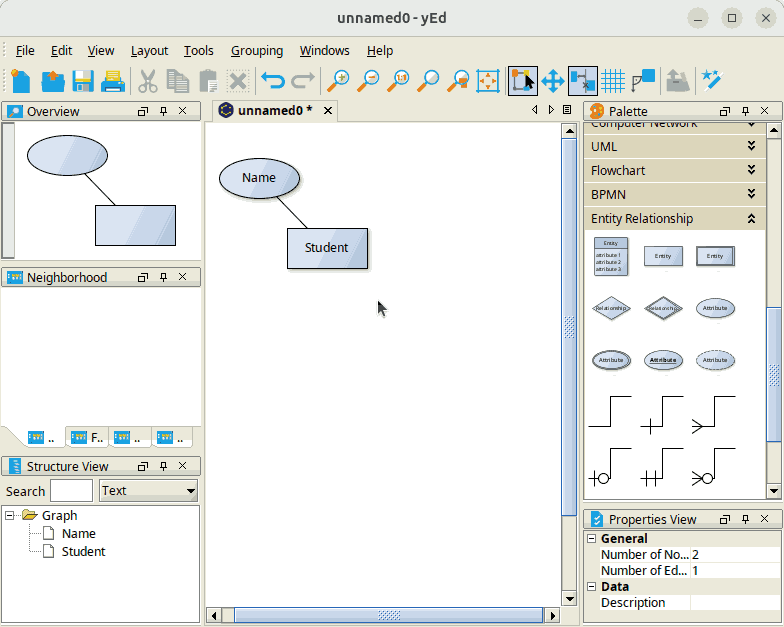
\includegraphics[width=0.48\linewidth]{\currentDir/yedErdEntitiesA13connectedToStudent}}}%
%
\floatSep%
%
\subfloat[][%
We add an attribute \emph{ID} in exactly the same way.%
\label{fig:yedErdEntitiesA14addedID}%
]{\tightbox{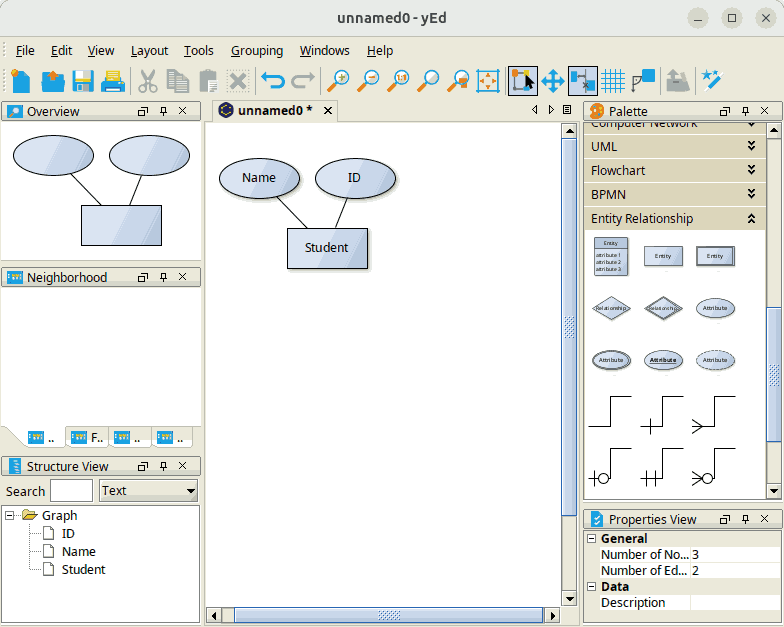
\includegraphics[width=0.48\linewidth]{\currentDir/yedErdEntitiesA14addedID}}}%
%
\floatRowSep
%
\subfloat[][%
We add several more attributes. %
Next, we click on the \menu{\underline{F}ile} menu.%
\label{fig:yedErdEntitiesA15addedAddrMobDoB}%
]{\tightbox{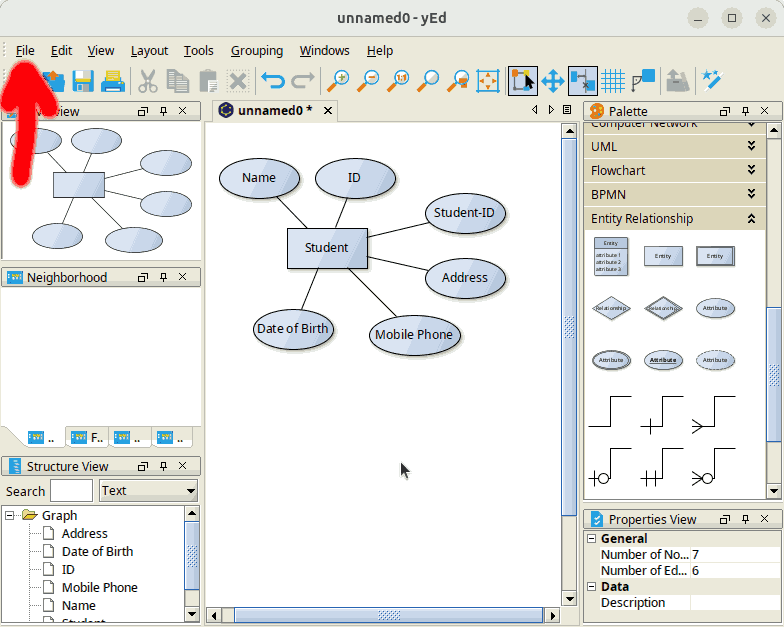
\includegraphics[width=0.48\linewidth]{\currentDir/yedErdEntitiesA15addedAddrMobDoB}}}%
%
\floatSep
%
\subfloat[][%
It is now time to save our document. %
We click on \menu{S\underline{a}ve As}.%
\label{fig:yedErdEntitiesA16saveAs}%
]{\tightbox{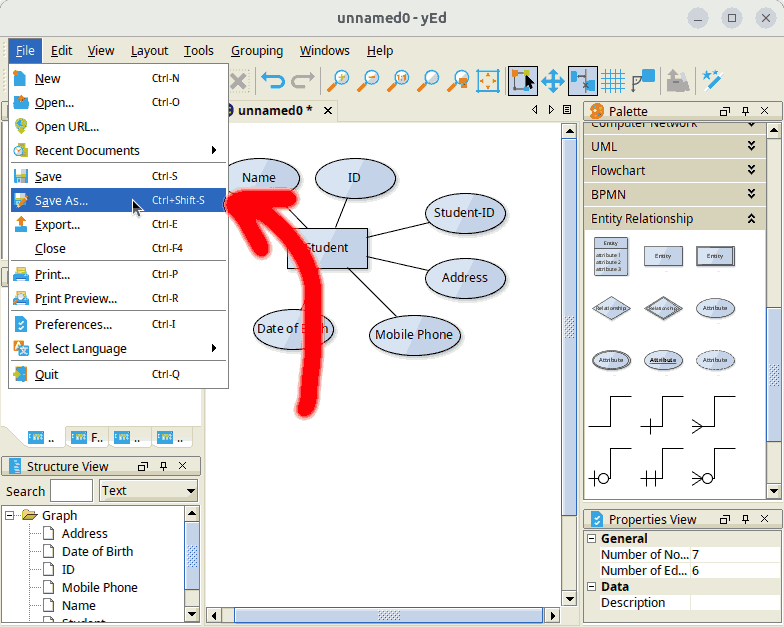
\includegraphics[width=0.48\linewidth]{\currentDir/yedErdEntitiesA16saveAs}}}%
%
\floatRowSep
%
\subfloat[][%
We save the diagram under the name \textil{erd_student_1} in the \textil{graphml} format by entering this name and clicking \menu{Save}.%
\label{fig:yedErdEntitiesA17saveAsErdStudent1}%
]{\tightbox{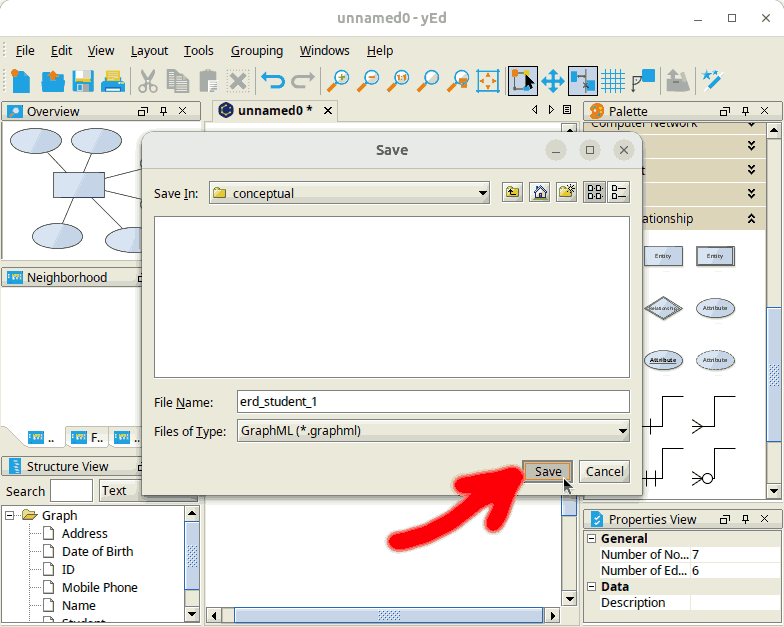
\includegraphics[width=0.48\linewidth]{\currentDir/yedErdEntitiesA17saveAsErdStudent1}}}%
%
\floatSep
%
\subfloat[][%
We can also store the diagram in a format that we can use in other documents. %
For this, we click on \menu{\underline{E}xport} in the \menu{\underline{F}ile} menu.%
\label{fig:yedErdEntitiesA18export}%
]{\tightbox{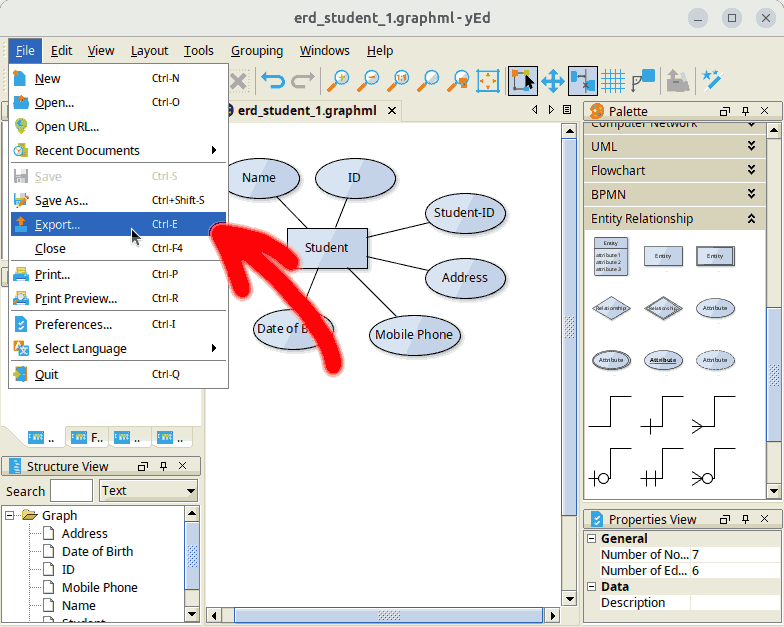
\includegraphics[width=0.48\linewidth]{\currentDir/yedErdEntitiesA18export}}}%
%
\caption{Drawing an \pgls{ERD} for the \emph{Student} entity using \yEd~(Continued).}%
\label{fig:yedErdEntitiesA:C}%
\end{figure}%
%
\begin{figure}%
\ContinuedFloat%
\centering%
%
\subfloat[][%
We choose to expert in the \pgls{SVG} format an click \menu{Save}.%
\label{fig:yedErdEntitiesA19exportToSvg}%
]{\tightbox{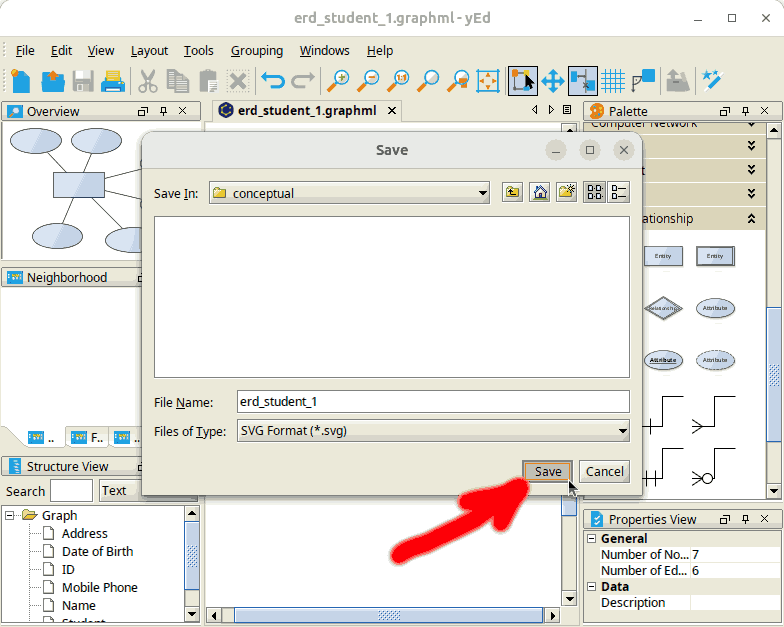
\includegraphics[width=0.48\linewidth]{\currentDir/yedErdEntitiesA19exportToSvg}}}%
%
\floatSep%
%
\subfloat[][%
We leave all settings as-is and click \menu{OK}.%
\label{fig:yedErdEntitiesA20exportToSvgDone}%
]{\tightbox{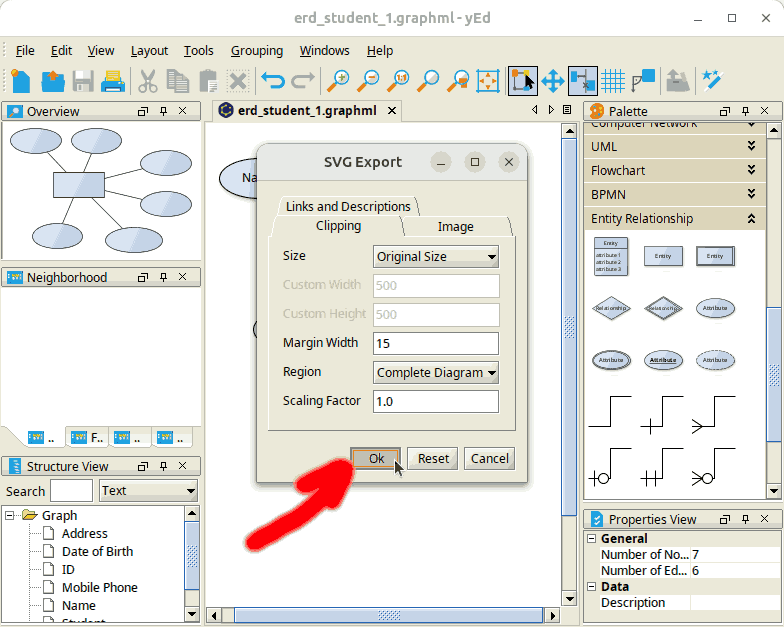
\includegraphics[width=0.48\linewidth]{\currentDir/yedErdEntitiesA20exportToSvgDone}}}%
%
\floatRowSep
%
\subfloat[][%
This produces this beautiful \pgls{ERD}.%
\label{fig:yedErdEntitiesA21erd}%
]{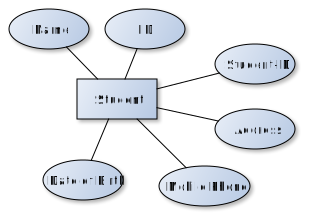
\includegraphics[scale=0.6]{\currentDir/yedErdEntitiesA21erd}}%
%
%
\caption{Drawing an \pgls{ERD} for the \emph{Student} entity using \yEd~(Continued).}%
\label{fig:yedErdEntitiesA:D}%
\end{figure}%

In the following sections, we will look at several different \pglspl{ERD}.
The goal of this course is to teach you \emph{actionable} knowledge.
So, while we will look at \pglspl{ERD}, we will also \emph{draw} them.
That, again, is fairly easy:
Once you understand the basic syntax, you can draw them with almost arbitrary drawing software.
Then again, this can also become tedious.
You could, for example, use the \softwareStyle{Draw} program which is part of \libreoffice, or a vector graphics program like \inkscape.
This would mean that you have to draw all the shapes of the diagrams independently, which would yield inconsistent designs and be generally tedious.
Then there are programs like \pgmodeler\ or \mysqlWorkbench\ which offer much better capabilities to draw \pglspl{ERD},
These tools, however, are bound to certain technologies, such as \postgresql\ and \mysql, respectively.
They would be useful for the development of logical models, but it feels awkward to apply them at a conceptual level, which should be technology agnostic.

After searching for a while, I have settled for \yEd~\cite{SG2015MDAWY,Y2011YGEM}.
\yEd\ is a free graph editor that offers a convenient ability to draw and layout \pglspl{ERD} while being entirely independent from any data model.
In \cref{sec:installingYed}, we provide instructions on how to obtain and install this program.
I will use it for all of the conceptual-level \pglspl{ERD} in the rest of the book.
As an example on how to use \yEd, we will give some instructions on how to draw the most simplest \pgls{ERD} with only a single entity inside in \cref{fig:yedErdEntitiesA:A}.
This program is rather easy to use, so after that example, we will assume that you can figure out how to draw more advanced \pglspl{ERD} on your own\dots
At least we do not just paint some \pglspl{ERD} and leave you entirely to your own devices when the time comes where you should draw some as well.

Before we really get into this, just a quick note:
In the context of \pglspl{ERD}, an \emph{entity type} are often called a \emph{entity}.
In other words, the meaning of the term \emph{entity} is shifted.
But let this not bother us too much.

The very first thing that we want to model is the entity (type) \emph{Student}.
From our requirements analysis, we know that students have names, they have an ID (issued by the government), they have a student ID (issued by our university), they have a mobile phone number, they have an address, and they have a \pgls{dateOfBirth}.
So let us model this.

After installing \yEd\ as discussed in \cref{sec:installingYed}, we open it.
We scroll down the \menu{Palette} pane on the right-hand side until we find the \menu{Entity Relationship} tab.
We click on the tab and it opens in \cref{fig:yedErdEntitiesA01scrollToErd}, offering us all the symbols and connectors commonly used in \pglspl{ERD}.
Entity (types) in \pglspl{ERD} are represented by rectangles.
We can now click on the \menu{Entity} symbol and drag it into the empty document in \cref{fig:yedErdEntitiesA02entity}.
We dragged the entity symbol into the diagram document in \cref{fig:yedErdEntitiesA03dragEntity}.

Inside the rectangle, the name of the entity (type) is written.
Let's change it to \inQuotes{Student}.
We therefore double-click into the new entity symbol in order to edit its name in \cref{fig:yedErdEntitiesA04doubleClickName}.
The text inside is marked.
We change the entity name to \inQuotes{Student} and press \keys{\enter} in \cref{fig:yedErdEntitiesA05changeNameToStudent}.
The name has changed.

Let us now add the attributes of the \emph{Student} entity step by step.
Attributes are represented as oval bubbles in \pglspl{ERD} that are connected to their owning entities by straight lines.
We now click on the \menu{Attribute} symbol in the element palette in \cref{fig:yedErdEntitiesA06nameIsStudentSelectAttribute}.
We drag the attribute symbol into our document in \cref{fig:yedErdEntitiesA07dragAttribute}.

Of course, in \cref{fig:yedErdEntitiesA08doubleClickName}, we want to change its name as well.
So we double-click into it to change its name.
We want its name to be, well, \inQuotes{Name,} i.e., we want to create an attribute that represents the name of the student in \cref{fig:yedErdEntitiesA09changeNameToName}.
We successfully changed the attribute name in \cref{fig:yedErdEntitiesA10changeNameChangedToNameSelectConnection}.
The attribute, however, is still floating in the diagram all by itself.
Attributes belong to entities, so we need to attach it to the entity \emph{Student}.

We thus now we click on the connection symbol in the palette and drag it right onto the attribute.
We drop the connection symbol onto the \emph{Name} attribute in \cref{fig:yedErdEntitiesA11dragConnection}.
Our mouse cursor now marks the end of a connecting line and we can drag the connection to whatever object we want to.
We click into the entity rectangle to connect the attribute \emph{Name} to the \emph{Student} entity in \cref{fig:yedErdEntitiesA12connectToStudent}.
The \emph{Name} attribute is now connected to the \emph{Student} entity in \cref{fig:yedErdEntitiesA13connectedToStudent}.

We add an attribute \emph{ID} in exactly the same way in \cref{fig:yedErdEntitiesA14addedID}.
We then go on and add several more attributes, \emph{Student-ID}, \emph{Address}, \emph{Mobile Phone}, \emph{\pgls{dateOfBirth}}, in \cref{fig:yedErdEntitiesA15addedAddrMobDoB}.
Notice that these are names that contain dashes and spaces, i.e., things that we would normally avoid when working with \sql.
But we are not working with \sql.
We are making a conceptual model.
We want this model to be easily readable and beautiful.
And it has to be.
Because we want to discuss it with our stakeholders.
So we do not need to heed to restrictions of a particular technology at this point in time.
Instead, we focus on readability.

Having finished drawing our very first \pgls{ERD}, it is time to save it.
Next, we click on the \menu{\underline{F}ile} menu.
We click on \menu{S\underline{a}ve As} in \cref{fig:yedErdEntitiesA16saveAs}.
We save the diagram under the name \textil{erd_student_1} in the \textil{graphml} format by entering this name and clicking \menu{Save} in \cref{fig:yedErdEntitiesA17saveAsErdStudent1}

We can open this file later in order to keep editing it.
However, we often want to also place the diagram into some document.
For this purpose, it makes sense to convert it to an image.
For this purpose, we click on \menu{\underline{E}xport} in the \menu{\underline{F}ile} menu in \cref{fig:yedErdEntitiesA18export}.
We choose to expert in the \glsreset{SVG}\pgls{SVG} format an click \menu{Save} in \cref{fig:yedErdEntitiesA19exportToSvg}.
In the dialog that pops up, we leave all settings as-is and click \menu{OK} in \cref{fig:yedErdEntitiesA20exportToSvgDone}.

This produces this beautiful \pgls{ERD} graphic shown in \cref{fig:yedErdEntitiesA21erd}.
Notice that we can also open the \pgls{SVG} graphic in other programs, such as \inkscape, to further edit and beautify it.
With this, we have completed our very first \pgls{ERD}.
(Although we did not yet really touch the \emph{Relationship} part symbolized by the \emph{R} in \pgls{ERD}.)

\usefulTool{yEd}{%
\yEd~\cite{SG2015MDAWY,Y2011YGEM} is a free graph editor that can be used to draw \pglspl{ERD}. %
It is useful for the conceptual modeling stage in \db\ design as discussed in \cref{sec:conceptualSchemaDesign}. %
Installation instructions are provided in \cref{sec:installingYed} and a small hands-on tutorial is given in \cref{sec:entitisAttrsErd}.%
}%
%
Anyway, let us continue our modeling adventure.
We take our \pgls{ERD} from \cref{fig:yedErdEntitiesA21erd} to our partners in the university, say, an administrator of one of the schools.
We want to discuss whether this model for students is appropriate.
During our discussion with the administrators, a few issues come up.

\begin{figure}%
\centering%
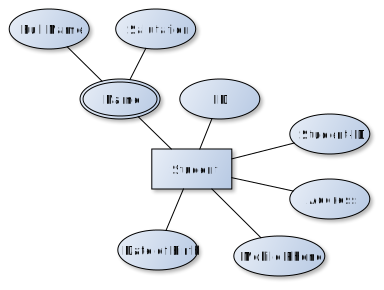
\includegraphics[scale=0.6]{\currentDir/erdStudent2}%
\caption{A new version of the \emph{Student} \pgls{ERD} from \cref{fig:yedErdEntitiesA21erd}, this time with \emph{Name} as composite attribute and \emph{Mobile Phone} as multi-valued attribute.}%
\label{fig:erdStudent2}%
\end{figure}%
%
First, \emph{Name}s are more complicated than we thought.
Students have a given name, a family name, and a salutation.
For example, the name of Mr.~Bebbo would actually be Mr.~Fred Bebbo, where \inQuotes{Bebbo} is the family name, \inQuotes{Fred} is the given name.
To accommodate this, \emph{Name} attribute should not be a single attribute.
We could turn it into a \emph{composite attribute}, consisting of given name, family name, and a salutation.
The system then could combine these components appropriately when addressing the student or when issuing documents.%
%
\begin{definition}[Composite Attribute]%
A \emph{composite attribute} is an attribute which consists of several parts with their own names and domains.%
\end{definition}%
\begin{definition}[Simple Attribute]%
A \emph{simple attribute} is an attribute that only has a single name and domain. %
Simple attributes do not have any components.%
\end{definition}%
%
%
When thinking about this, we encounter a problem:
In Western culture, the full name is composed by first writing the given name and then the family name.
This is why the full name of Mr.~Bebbo is Fred Bebbo.
In Eastern cultures, it is the other way around:
The name of the famous Chinese mathematician 刘徽 is transcribed as LIU Hui in the Latin alphabet.
LIU~(刘) here is the family name and it comes first.
Hui~(徽) is the given name and it comes second.
Depending on the cultural background, the system would need to decide how to compose the name correctly.
This sounds a like an awful problem that would probably become the source of many interesting errors or, at least, complaints.

We decide to not compose the name of given name and family name.
Instead, we provide two values as part of the \emph{Name} attribute:
The \emph{Full Name} will be the complete and official name, as written on the ID card.
This would be something like 刘徽 for a Chinese person and Fred Bebbo for the Westerner Mr.~Bebbo.
As second component, we store the \emph{Salutation}.
For 刘徽, this could be 刘教授 and for Fred Bebbo, it could be Mr.~Bebbo.
Maybe we could later permit the students to change their salutation in the system to whatever they feel comfortable with.
The full name, however, would be entered by an administrator exactly as it is spelled on the student's ID document.
If our system would ever sent an automated message to Mr.~Bebbo, it will use the salutation.
If we print the name on a certificate, we will use the full name.
A composite attribute in the \pgls{ERD} is simply drawn with the components as attributes connected to the attribute.

We also notice that a student may have multiple mobile phone numbers.
Such multi-valued attributes can be modeled by ellipses with small ellipses inside.%
%
\begin{definition}[Multi-Valued Attribute]%
An entity may have multiple values for a \emph{multi-valued attribute}.%
\end{definition}%
\begin{definition}[Single-Valued Attribute]%
An entity has (at most) one value for a \emph{single-valued} attribute.%
\end{definition}%
\begin{definition}[Optional Attribute]%
An entity may or may not have a value for an \emph{optional attribute}. %
If an attribute has no value, this is often represented as \sqlilIdx{NULL}.%
\end{definition}%
%
A single-valued optional attribute has either one value or no value.
A single-valued non-optional attribute has exactly one value.
A multi-value optional value has either no value, one value, or multiple values.
A multi-valued non-optional attribute has one value or multiple values.

Upon closer inspection, we notice that the mobile phone number attribute should probably be modeled as optional multi-valued attribute.
While it seems very unlikely nowadays, there may be students who do not have a mobile phone number.
Well, maybe a foreign exchange student, i.e., a 留学生, who enters China does not yet have a mobile phone number when enrolling into our university.
So making this attribute optional is reasonable.

While we are on the subject of foreign exchange students:
They probably do not have a Chinese ID.
So we turn ID into an optional single-valued attribute.
Optional attributes can be signified by small empty bubbles at the end of the lines connecting them to the entity types.

We update our \pgls{ERD} in \cref{fig:erdStudent2}.
The \pgls{dbs} could now decide whether to fully spell out the name, e.g., in graduation certificates, or whether to just print the salutation and family name, e.g., when sending messages addressed to the students.
Now we also are able to represent that fact that a student can have no or multiple mobile phone numbers.
They also can have no or one ID.

\begin{figure}%
\centering%
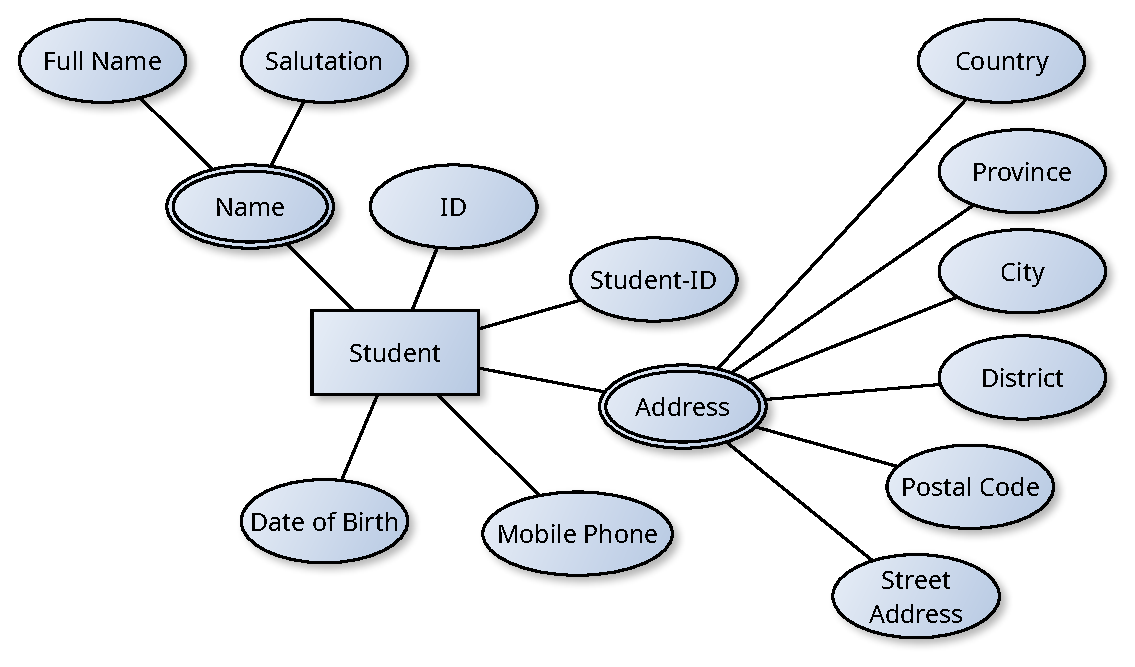
\includegraphics[scale=0.6]{\currentDir/erdStudent3}%
\caption{A new version of the \emph{Student} \pgls{ERD} from \cref{fig:erdStudent2}, this time with \emph{Address} as multi-valued \emph{and} composite attribute.}%
\label{fig:erdStudent3}%
\end{figure}%
%
While we are at this, we realize that \emph{Address} should also be a composite attribute.
An address is not just a line of text, but consists of components such as country, province, city, district, postal code, street and street number, quarter, building, and flat number.
Modeling that would be cumbersome.
We propose that everything after the postal code could simply be merged into one string named \emph{street address}, because an automated system probably cannot really handle information at a finer granularity than postal code in any meaningful way.
While discussing the subject with our partners, we also realize that \emph{Address} should be a multi-valued attribute, i.e., a student can have multiple addresses.
This is illustrated in \cref{fig:erdStudent3}.

\begin{figure}%
\centering%
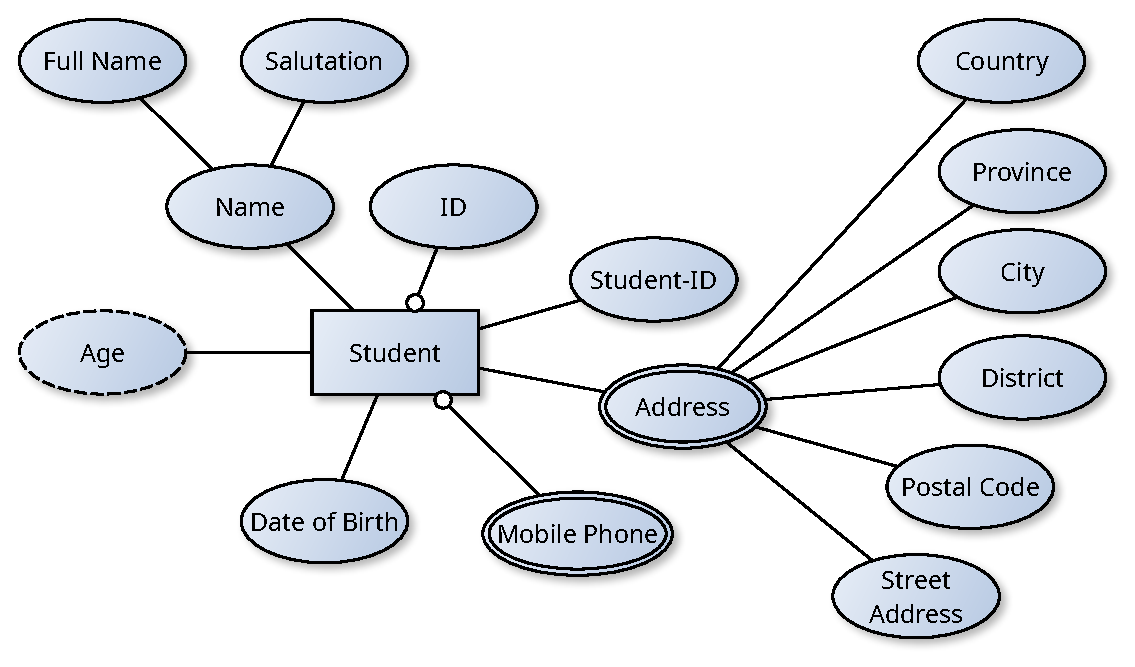
\includegraphics[scale=0.6]{\currentDir/erdStudent4}%
\caption{A new version of the \emph{Student} \pgls{ERD} from \cref{fig:erdStudent3}, where we added the derived attribute \emph{Age}.}%
\label{fig:erdStudent4}%
\end{figure}%

Finally, there are also so-called derived attributes.
A derived attribute is calculated based on the values of other attributes.
It does not need to be stored in the \db.
A typical example is the age of person.
If we know the \pgls{dateOfBirth} and the current date, the age can directly be calculated.
This can be done very quickly.
There is no reason to store the age in the \db.
Derived attributes are illustrated by ellipses with dashed lines around thei perimeter, as shown in \cref{fig:erdStudent4}.

At this stage, we have learned several things about entities and attributes.
An entity models some real-world object, person, thing, location, event, or concept.
An entity does not just exist.
It is the merger of its attribute values.

Attributes can have different properties as well~\cite{S2024D:CDMERDE}:
Attributes can be \emph{simple}, which means that they have atomic values that cannot be subdivided any further, like phone numbers.
Attributes can be \emph{composite}, which means that they consist of parts.
An address, for example, can be divided into country, province, city, etc.

It is not always immediately clear how an attribute could be modeled.
For example, our students have the attribute \glsreset{dateOfBirth}\emph{\pgls{dateOfBirth}}.
Technically, we have learned back in \cref{sec:factory:demand} that dates are atomic datatypes in \sql.
So naturally, we would model the \pgls{dateOfBirth} as an atomic attribute.
Of course, we could also model it as a composite attribute consisting of year, month, and day.
Then again, an address could also be represented as a single string of text instead of using a composite attribute.

The decision of how to model attributes probably depends on which data we need.
For example, if we store dates as, well, atomic dates, then it is extremely easy and fast to calculate the year of birth or the age of a person.
Storing years separately would be useless and just complicate and slow down the \db.
For an address, however, extracting the country from an address string could be tedious and error prone.
And we would probably need the country in almost any use case where an address is required.

Anyway, besides being either simple or composite, attributes can also be single-valued or multi-values.
Students can have multiple addresses, multiple phone numbers, but only a single \pgls{dateOfBirth}.%
\FloatBarrier%
\endhsection%
%
